\section{Battery selection}
\label{Chap:Battery_Selection}
In the current Solar Jet project, the Schübeler 7800 HDME battery has been chosen as the energy carrier unit. A detailed argumentation is lacking however. In this section therefore it is investigated what the battery requirements are for the set goal of the project. A battery selection process will then finally decide upon a suitable battery.
\subsection{Requirements}
\begin{enumerate}
\item Energy\\
The Solar Jet project's short term goal is to set a speed of 450\textit{km/u}. In a previous bachelor thesis of Jasper Oranje \cite{BEP_Jasper} it is noted that this speed is only achievable for a short amount of time because of the EDF heating up. For the energy required, it is then assumed that the Solar Jet has to be able to fly at a cruising speed of 394\textit{km/u} for up to three minutes. With an energy transmission efficiency of 0.7, it is now calculated that the battery needs 547.22\textit{Wh}. This only accounts for overcoming the drag force, and does not take into account the energy needed for acceleration.\\
For the EDF to thrust full power, it draws around 9000\textit{W} and requires a voltage of approximately 50\textit{V}. The current draw can now be calculated from equation \ref{Eq:current_draw}.
\begin{equation}
\label{Eq:current_draw}
I = \frac{P}{V} = \frac{9000}{50} = 180 \textit{A}
\end{equation}
With this, the voltage, the current and the capacity needed have been determined.
\item Safety\\
Lithium-ion batteries are vulnerable to safety issues and can violently decompose when these are not met. The battery should therefore never exceed safety margins set by the manufacturer, which usually include a thermal operating range, a voltage operating range and a maximal charge and discharge current as described in section \ref{Chap:Battery_Safety}.\\
Furthermore the battery should be able to handle crashes. Especially with pouch cells, a construction has to be created to handle mechanical impact preventing internal short-circuit, since a hard-metal casing is non-present.
\item Other\\
Lastly, there are three more aspects. The battery should be as light as possible, as every addition of weight requires more thrust to accelerate. Besides weight, the battery should be dimensioned proportionally so that it fits in the allocated design space. Finally, the battery must be practical: The battery has to be easily removable from the Solar Jet for charging or inspection. The battery assembly from the individual cells must be manageable as well.
\end{enumerate}
\subsubsection{Cylindrical versus Pouch}
The first decision to make is whether to use cylindrical cells or pouch cells. Cylindrical cells come with safety, but also come with complexity, weight and volume. Pouch cells on the other hand come with energy density and relative simplicity, but might be prone to failure.

\textit{Cylindrical cell battery pack}\\
Cylindrical lithium-ion cells come in several sizes, but the 18650 size is almost exclusively used. 18650 stands for 18\textit{mm} in diameter, and 650\textit{mm} in length. Since the size is standardized, the range of options shrinks dramatically. There is only a few select creditable manufacturers and only a few select of chemistries to choose from. To further decrease this list of viable options, the influence of energy requirements has to be checked. 18650 cells always have a nominal voltage of 3.6\textit{V}. This means 14 battery packages in series for the required 50\textit{V} voltage. For the current, 180\textit{A} is needed for the EDF. 18650 batteries can not handle currents of 180\textit{A}, and thus need to be switched in parallel. The amount depends on the maximal current one cell is able to handle. In table \ref{Table:18650_cell_comparison} three option are listed plus an additional battery. Battery info comes from Batterybro \cite{Batterybro}, a 18650 cell vendor that sells top brand batteries, include the manufacturers spreadsheet and rate the batteries themselves aswell to correct for 'enthusiastic' spreadsheets.
\begin{table}[H]
\centering
\caption{18650 cell package needed for 50\textit{V}, 180\textit{A}}
\label{Table:18650_cell_comparison}
\begin{tabular}{|l|l|l|l|l|l|}
\hline
Battery & Current(\textit{A}) & Capacity(\textit{Ah}) & Package & Total capacity(\textit{Wh}) & Total weight(\textit{kg}) \\
\hline\hline
1. Sony VTC4			& 30			& 2							& 14S6P  & 604.8 & 3.780\\ \hline
2. LG Chem HB6			& 30				& 1.5				    & 14S6P & 453.6 & 4.032	 \\ \hline
3. Samsung INR-25R5			& 20			& 2.5			    & 14S9P & 1134 & 5.670\\ \hline
4. Panasonic NCR-B			& 5			& 3.4			    & 14S36P & 6168.96 & 22.780\\ \hline
\end{tabular}
\end{table} 

\subsection{Selecting a battery}
\label{Selecting_A_Battery}

%\begin{figure} [H]
% 	\centering
% 	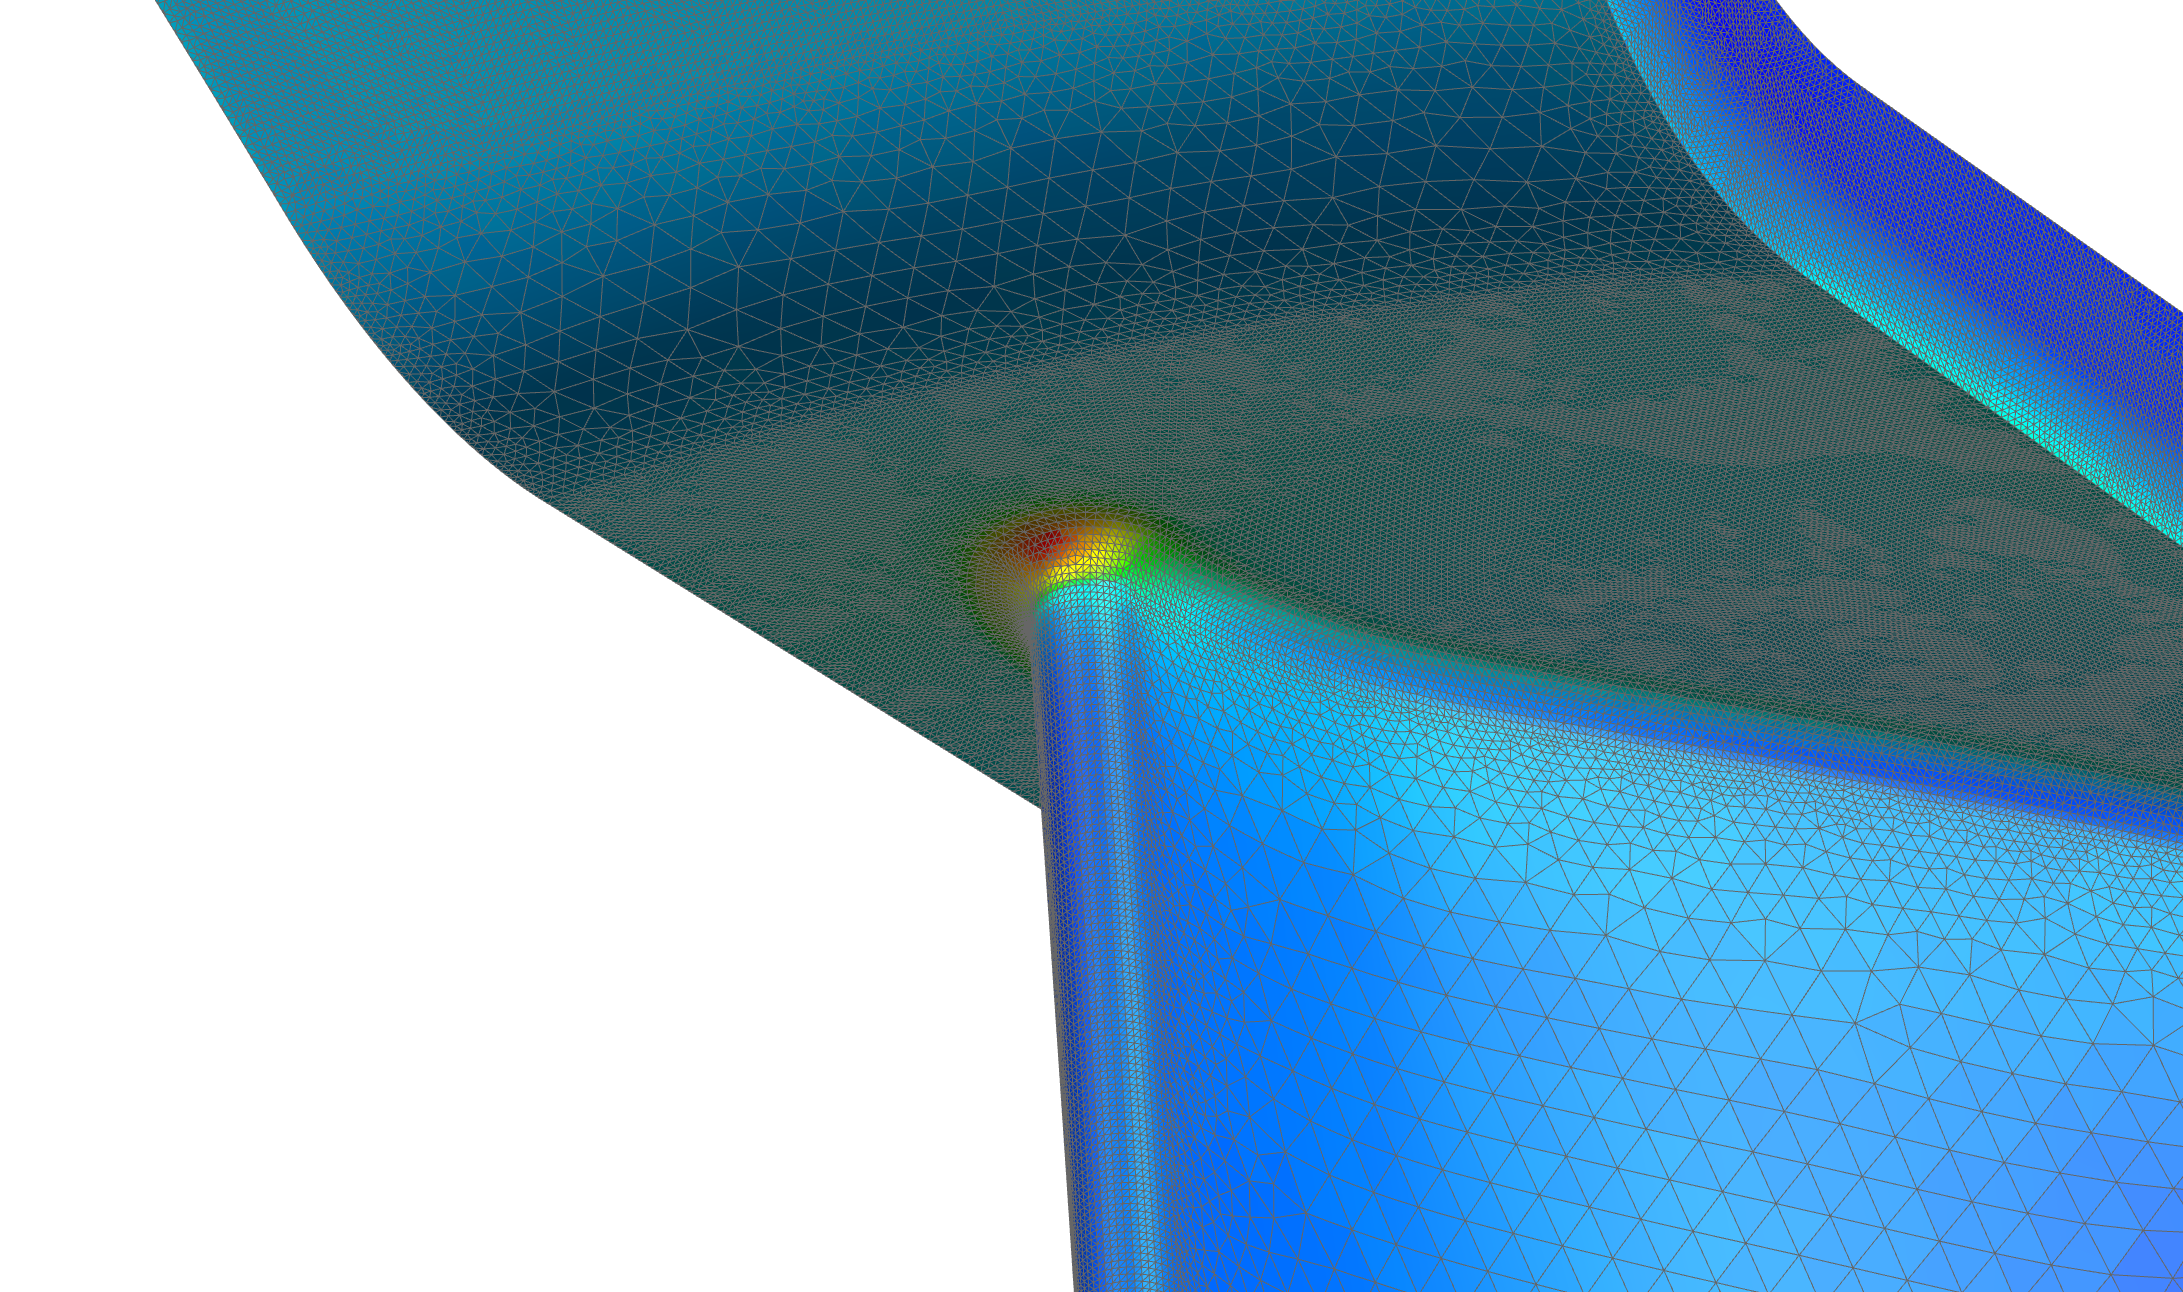
\includegraphics[width=0.8\linewidth]{Figures/stator_shutdown.png}
% 	\caption{Maximum stress during shut-down condition}
%    \label{stator1}
% \end{figure}

\newpage